\subsection{Daglig helbredstilstand}
Førend en træning påbegyndes skal brugerens daglige helbredstilstand angives. Dette er for at sikre, at træningen tilpasses den individuelle bruger samt imødekomme dag til dag variationer. Af \autoref{fig:helbredstilstand} fremgår aktivitetsdiagrammet for den daglige helbredstilstand. 

\begin{figure} [H]
\centering
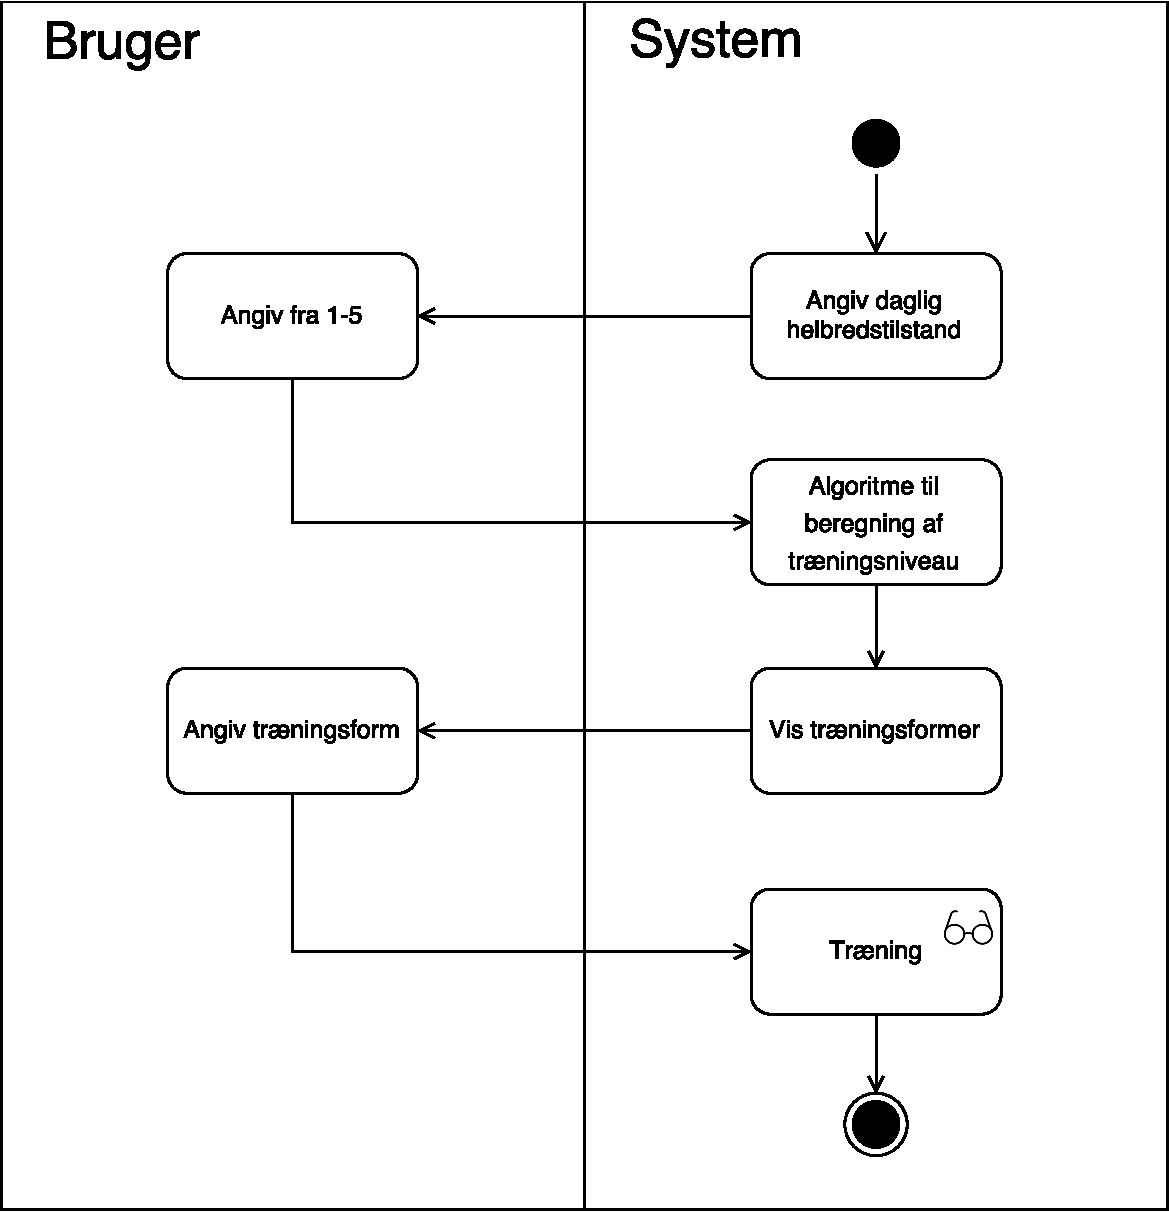
\includegraphics[width=0.9\textwidth]{figures/aktivitetsdiagram/Helbredstilstand}
\caption{Aktivitetsdiagram for daglig helbredstilstand.}
\label{fig:helbredstilstand}
\end{figure}

Den dagelige helbredtilstand angives ved hjælp af en skala fra et (dårlig helbredstilstand) til fem (god helbredstilstand). Ud fra den daglig helbredstilstand, kategoriseringen af KOL samt evaluering fra førhenværende træning, passende til det angivet helbredstilstand, vælges et træningniveau passende til brugerens nuværende helbred. Dertil foreslås brugeren forskellige træningsformer, herunder konditions-, styrketræning samt vejrtrækningsøvelser. Den ønskede træningsform vælges, hvortil træningen kan initieres. Træningen er yderligere beskrevet i \autoref{sec:traening}. 
